\RequirePackage{fix-cm}
\documentclass[twocolumn]{svjour3} 
\smartqed 
\usepackage{graphicx}
\tolerance=1
\emergencystretch=\maxdimen
\hyphenpenalty=10000
\hbadness=10000
\def\makeheadbox{\relax}
\usepackage[numbers]{natbib}
\usepackage{algorithm,algorithmic}
\renewcommand{\algorithmicrequire}{\textbf{Input:}}
\renewcommand{\algorithmicensure}{\textbf{Output:}}
\usepackage{amsmath,amssymb}
\usepackage{tabularx}
\usepackage{ntheorem}
\newtheorem{defn}{Definition}
\usepackage{tikz}
\usetikzlibrary{arrows.meta, positioning, shapes.geometric}
\usepackage{color}
\usepackage{latexsym}
\usepackage{enumitem}
\usepackage{algorithm}
\usepackage{algpseudocode}
\usepackage{amsmath}
\renewcommand{\algorithmicrequire}{\textbf{Input:}}
\renewcommand{\algorithmicensure}{\textbf{Output:}}

\usepackage{mathptmx}
\emergencystretch=\maxdimen
\hyphenpenalty=10000
\hbadness=10000
\usepackage{tikz}
\usetikzlibrary{decorations.pathreplacing}
\usepackage{pgfplots}
\usetikzlibrary{shapes.geometric, arrows,patterns,calc}
\tikzstyle{startstop} = [rectangle, rounded corners, minimum width=3cm, minimum height=1cm,text centered, draw=black, fill=red!30]
\tikzstyle{io} = [trapezium, trapezium left angle=70, trapezium right angle=110, minimum width=3cm, minimum height=1cm, text centered, text width=3cm, draw=black, fill=blue!30]
\tikzstyle{process} = [rectangle, minimum width=4cm, minimum height=0.8cm, text centered, text width=4cm, draw=black, fill=orange!30]
\tikzstyle{decision} = [diamond, aspect=3, minimum width=2cm, minimum height=0cm, text badly centered, text width=3cm, draw=black, fill=green!20, inner sep=0pt]
\tikzstyle{line} =[draw, thick, -latex,shorten >=2pt]
\tikzstyle{arrow} = [thick,->,>=stealth]
\tikzstyle{end} = [ellipse,draw=black,fill=blue!30,text badly centered,minimum height=2em]
\pgfplotsset{compat=1.12}
%% Magnify a portion in tikz using spy
\usetikzlibrary{spy}
\usetikzlibrary{backgrounds}
\usetikzlibrary{decorations}


\begin{document}

\title{From User Needs to Accurate Rankings: A Multi-Criteria Framework for Cloud Service Provider Selection}

\titlerunning{Data-Centric Cloud Service Selection}        

\author{
Arup Kumar Harichandan \and
Rakesh Ranjan Kumar \and
Debendra Muduli \and
Soumya Snigdha Mohapatra
}
\authorrunning{Kumar et al.}
\institute{
Arup Kumar Harichandan \at
Department of Computer Science and Engineering, \\
C V Raman Global University, Bhubaneswar 752054, India \\
\email{arup.harichandan@gmail.com}
\and
Rakesh Ranjan Kumar* (Corresponding Author) \at
Department of Computer Science and Engineering, \\
C V Raman Global University, Bhubaneswar 752054, India \\
\email{rakeshranjan@cgu-odisha.ac.in}
\and
Debendra Muduli \at
Department of Computer Science and Engineering, \\
C V Raman Global University, Bhubaneswar 752054, India \\
\email{debendra.muduli@cgu-odisha.ac.in}
\and
Soumya Snigdha Mohapatra \at
Department of Information Technology, \\
Pillai College of Engineering, Mahatma Education Society, \\
New Panvel, Navi Mumbai 410206, India \\
\email{soumyamohapatra@mes.ac.in}
}


\date{}
% The correct dates will be entered by the editor


\maketitle

\begin{abstract}
In today’s cloud-driven world, choosing the right cloud service provider (CSP) is a complex decision because it involves balancing multiple technical and business requirements. Many existing methods for CSP selection focus on objective criteria, but fail to clearly connect user needs to how providers are finally ranked. This paper introduces a framework that combines Analytic Hierarchy Process (AHP), Quality Function Deployment (QFD) and Technique for Order Preference by Similarity to Ideal Solution (TOPSIS) to bridge this gap. By mapping user-defined requirements to QoS attributes through QFD, the approach ensures that the rankings reflect what users actually value. The framework is tested on real CSP performance data and compared with AHP--TOPSIS, MOORA, and VIKOR. It achieves better ranking accuracy and stronger alignment with user priorities. Robustness is validated using Kendall’s Tau, Wilcoxon tests, RMSE, MAE, and sensitivity checks on the variation of the QFD scale. An execution time study shows that the entire process remains efficient, taking less than a second even for 50 CSPs and 10 attributes. These results confirm that the proposed approach is both practical and easy to interpret for real-world CSP decisions.
\end{abstract}

\keywords{Cloud Service Selection \and Quality of Service  \and MCDM   \and QFD \and AHP \and TOPSIS }



\section{Introduction}

Cloud computing has become the backbone of modern digital services, offering flexible and on-demand access to computing resources~\cite{varghese2018next,phaphoom2013foundations}. However, selecting the most suitable cloud service provider (CSP) is not straightforward. Different users place importance on different aspects, such as cost, security, availability, or scalability, making it a multi-criteria decision-making problem. Traditional approaches like AHP, TOPSIS, MOORA, and VIKOR can rank providers systematically, but they rarely explain how user-defined requirements influence the final ranking. Many studies also overlook important robustness checks, such as sensitivity analysis or execution time assessment, which are vital to confirm that a framework can perform reliably when applied to larger datasets and real-world scenarios~\cite{garg2013framework, hussain2022cloud,kumar2017prioritizing}.

In real world settings, cloud users typically have different functional requirements, such as low response time, high availability, secure data handling, and cost effectiveness, that need to be systematically mapped to the Quality of Service (QoS) attributes provided by various vendors~\cite{kumar2021ccs,tiwari2021g}. But in reality, the variety and constant changes in cloud environments make this mapping far from straightforward. As applications become more complex, users also expect greater clarity and finer control over how services are evaluated and selected. Most traditional cloud service selection methods use multi-criteria decision-making (MCDM) techniques, where experts assign weights to QoS criteria. Although this can work in well-defined situations, it often introduces subjectivity, uneven weight assignments, and limited transparency in how user needs are transformed into measurable metrics~\cite{mostafa2022hybrid}.

Several frameworks have used methods like AHP, TOPSIS, VIKOR, and similar techniques to rank cloud services. However, many of these models do not capture the voice of the customer in a meaningful way~\cite{opricovic2004compromise,thakur2022cloud}. In most cases, QoS attributes are treated in isolation, without linking them to what users actually need. Some studies even assume equal weights or focus only on technical performance, overlooking the context in which services are used. Although entropy-based and machine learning-driven models aim to bring more objectivity, they still struggle to provide clear traceability between user needs and how providers are evaluated~\cite{liu2020heterogeneous,monika2022framework}. As a result, there is often a gap between user priorities and the final rankings. In addition, most existing approaches rely on static weights, rarely validate their results statistically, and tend to focus on optimization accuracy rather than aligning decisions with user requirements. These gaps highlight the need for a structured decision-making framework that directly links user-defined functional requirements to measurable QoS attributes and validates provider rankings through robust statistical and sensitivity analyses.


These limitations highlight the need for a transparent, data-driven, and user-centric selection framework that minimizes subjective interference while maintaining strong alignment between requirements and evaluation. We first apply AHP to determine the relative importance of user-defined functional requirements. These prioritized requirements are then used within the QFD framework to compute the derived weights for the objective QoS attributes~\cite{sousa2017qfd}. The final ranking of cloud service providers is obtained using the TOPSIS method, based on normalized performance scores and these QFD-derived weights.

A comprehensive case study involving ten real-world cloud providers is conducted using online performance data. To validate the robustness of the model, comparative experiments are performed against several baseline MCDM techniques, including AHP-TOPSIS, MOORA, and VIKOR. In addition, statistical significance tests are performed using Kendall's Tau and Wilcoxon signed rank tests to ensure the reliability of the observed ranking differences.

The key contributions of this study are summarized as follows:
\begin{itemize}
    \item We develop a practical decision-making framework that combines AHP, QFD, and TOPSIS to create a clear connection between what users need and how cloud providers are evaluated.
    \item The framework uses QFD to translate user priorities into measurable QoS weights, making the decision process more transparent and less subjective than many existing methods.
    \item We demonstrate the framework using real performance data from ten cloud service providers, instead of relying only on simulated or hypothetical datasets.
    \item Through comparisons with AHP-TOPSIS, MOORA, and VIKOR, we show that incorporating user requirements in the weighting process leads to more meaningful and user-focused rankings.
    \item The model is tested using multiple validation methods, including Kendall's Tau, Wilcoxon's signed rank test, RMSE, MAE, and sensitivity analysis. This goes beyond the basic rank correlation checks that most existing studies use.
    \item We highlight the drawbacks of current dynamic and machine learning-based models, such as limited interpretability and weak traceability of user needs, and explain how our framework overcomes these issues while staying scalable and easy to implement.
\end{itemize}


To guide the reader, the remainder of this paper is organized as follows. Section 2 presents related work in the area of cloud service selection and highlights gaps in existing approaches. Section 3 introduces the proposed QFD-AHP-TOPSIS framework, including the methodology for requirement mapping, weight derivation, and service classification. Section 4 describes the case study conducted using data from real-world cloud providers and presents the results. Section 5 discusses statistical validation with multiple tests. Finally, Section 6 concludes the paper with key findings and future directions.

\section{Related Work}

Cloud service selection (CSS) has emerged as a critical multi-criteria decision making (MCDM) challenge, driven by the increasing complexity, heterogeneity, and scale of cloud offerings. Various frameworks have been proposed to help select optimal cloud service providers (CSPs), primarily using quantitative decision models such as AHP, TOPSIS, VIKOR and their hybrids~\cite{whaiduzzaman2014cloud,sun2019framework}. These models typically aim to balance trade-offs between performance, availability, cost, and other quality of service (QoS) parameters. However, a significant share of these efforts are often grounded in subjective weight assignment, limited scenario validation, or lack a robust link between user requirements and provider capabilities~\cite{vakili2019cloud,sun2016cloud}.



\begin{table*}[t]
\centering
\caption{Comparative Summary of Recent Cloud Service Selection Models}
\label{tab:comparison}
\scriptsize
\begin{tabular}{|p{2.9cm}|p{2.5cm}|p{2.1cm}|p{2.1cm}|p{2.3cm}|p{2.2cm}|}
\hline
\textbf{Reference} & \textbf{Methodology} & \textbf{Weight Derivation} & \textbf{QoS Source} & \textbf{Validation} & \textbf{Limitation} \\
\hline
Paper ~\cite{bhol2024machine} & AHP + VIKOR + Entropy & Hybrid & Real + Estimated & Kendall Tau & No link to functional needs \\
\hline
Paper~\cite{chauhan2025fbm} & Fuzzy Brokering Model & User feedback (linguistic) & Subjective & Execution metrics only & No robustness or traceability \\
\hline
Paper ~\cite{li2023multi} & Monte Carlo Tree Search & Not specified & Real-time system states & Accuracy, latency & Optimization-centric \\
\hline
Paper ~\cite{tang2024two} & Trust-aware recommender & Historical similarity & Behavior logs & Precision/Recall & No QoS-functional alignment \\
\hline
Paper~\cite{hussain2022cloud} & BWM + Markov Fusion & Mixed (expert + entropy) & Benchmarks + surveys & Kendall, Sensitivity & No user-centered criteria design \\
\hline
Paper~\cite{gireesha2022fuzzy} & Fuzzy-MADM & Linguistic weights & Simulated data & Case outcome only & No formal consistency checks \\
\hline
Paper~\cite{bi2022cloud} & Weighted KD-tree & Static scoring functions & Simulated profiles & Ranking accuracy & No dynamic mapping logic \\
\hline
Paper~\cite{tomar2023decision} & AHP-TOPSIS variants & Subjective AHP & Simulated or benchmark & Correlation-based & Assumes expert-consistent priorities \\
\hline
Paper~\cite{kumar2017prioritizing}} & AHP + COPRAS & Pairwise judgments & Expert preference & Direct scores & No sensitivity/statistical validation \\
\hline
Paper ~\cite{raghavan2021membrane} & Membrane Model & Quantitative encoding & Objective measures & Pareto optimality & Lacks interpretability and ranking stability \\
\hline
Proposed Work (This Paper) & AHP + QFD + TOPSIS & AHP-based requirement weights + QFD-derived QoS weights &Real-world CSP data & ReKendall’s Tau, Wilcoxon test, RMSE, MAE, Sensitivity analysis & Addresses gaps by: (i) linking user-defined functional needs to QoS attributes, (ii) reducing subjectivity in weight assignment, (iii) performing robust statistical and sensitivity validation using real data. \\
\hline
\end{tabular}
\end{table*}


The early work of 2015-2017 laid the foundation for subsequent advancements. For example, the paper~\cite{jatoth2017evaluating} adopted an DEA-based model using expert-derived weights to prioritize CSPs, but their static data assumptions limited scalability. In paper ~\cite{boutkhoum2016selection} applied PROMETHEE to classify providers based on service level agreements, yet their work lacked feedback-driven weight updates. In paper~\cite{kumar2016evaluation}, a fuzzy hybrid AHP-TOPSIS model was proposed, improving uncertainty handling, although it omitted empirical validation under dynamic QoS conditions.

Continuing into 2018-2020,~\cite{wang2019cloud} combined AHP with GRA (Gray Relational Analysis), demonstrating better classification consistency but lacking performance-optimal mapping. Hussain et al. present a smart decision-making framework that helps organizations choose the best cloud service by carefully weighing multiple important factors~\cite{hussain2020novel} . The paper~\cite{hussain2022cloud} introduces a new cloud service selection framework (C3SF) that guides users step by step: from gathering their needs to analyzing, evaluating and finally reaching a shared decision on the best service. The paper ~\cite{tiwari2021g} proposes GTOPSIS, an improved method to rank cloud services more reliably by tackling the rank-reversal issue using a Gaussian distribution. Although it improves accuracy using real-world data, challenges such as handling dynamic QoS changes and user-specific preferences remain. The paper ~\cite{youssef2020integrated} offers a smarter way to choose cloud services by combining BWM and TOPSIS for more consistent decision making. But it still fails in handling changing user needs or how different criteria might affect each other in real-world situations.

In one widely cited work, ~\cite{nawaz2018mcdm} tackles the challenge of shifting user preferences in cloud service selection by using a Markov chain to model changes and BWM to rank services, showing better results than AHP. However, it still lacks deeper explainability and adaptability to rapidly changing or highly personalized user needs. ~\cite{chauhan2025fbm} introduced a Fuzzy Brokering Model (FBM) for federated clouds, using user feedback in linguistic terms. Although the approach captured uncertainty, it failed to validate robustness through rank sensitivity or efficiency measures. Similarly, Gireesha et al.'s fuzzy-MADM approach prioritized linguistic modeling but did not establish a mechanism to ensure consistency of service ranking under varied QoS profiles~\cite{gireesha2022fuzzy}.

Several recent models have begun to integrate hybrid or learning-based methods for selecting dynamic or context-sensitive services. Li et al. implemented a two-layer Restricted Monte Carlo Tree Search for multi-cloud brokering, demonstrating high efficiency in service decision latency, although it focused on optimization logic rather than requirements alignment~\cite{li2023multi}. Tang et al. proposed a trust and similarity-enhanced model for service recommendation, offering precision-based validation but limiting the decision framework to user behavior data~\cite{tang2024two}. 



In addition to algorithmic limitations, many existing models also lack rigorous statistical validation. Although Kendall's Tau or simple rank correlation is occasionally used, few works provide a comprehensive battery of robustness tests, such as Wilcoxon signed-rank, sensitivity analysis, or rank reversal evaluation. Execution time or computational complexity, a key concern in scalable and real-time cloud systems, is often ignored or under-reported. Furthermore, while simulation-based datasets or expert-derived rankings are common, relatively few models are validated using real-time or benchmark performance repositories such as CloudHarmony.Furthermore, most selection strategies still operate under isolated user or single-tenant assumptions. Very few consider the evolving functional needs of users or support modular updates to decision matrices without full re-evaluation. There is also a lack of semantic traceability between functional requirements and evaluation scores, leading to limited interpretability for stakeholders.

Although prior work offers mathematical rigor and hybrid models, they often lack a clear mapping between user-defined functional requirements and technical QoS indicators. Many rely on static weighting, isolate QoS from user context, or overlook statistical validation. Our proposed model addresses these limitations by using QFD as the core structure, with AHP applied to prioritize user requirements within the QFD matrix. These priorities are translated into QoS weights, enabling TOPSIS-based provider ranking. This integrated, requirement-aware, and data-driven approach ensures semantic traceability, transparency, and robustness, marking a significant step forward over the existing literature.

\subsection{AHP in related Work}
The Analytic Hierarchy Process (AHP), proposed by Saaty, is widely used to structure and quantify decision problems that involve subjective judgments~\cite{saaty2004decision}. In the domain of cloud service selection, AHP has been applied to determine the relative importance of various evaluation criteria such as cost, availability, and performance. Most existing approaches use AHP to capture user preferences through pairwise comparisons and then assign static weights to QoS attributes ~\cite{kumar2018novel,saha2021hybrid,tiwari2021g}. Although effective, these models often stop at the criteria level and do not account for deeper user-driven requirements. Our work builds on this foundation by applying AHP at the requirement level, ensuring that functional needs defined by users are prioritized before being translated into technical attributes via QFD.

\subsection{QFD in related Work}
Quality Function Deployment (QFD) is a structured approach to translate customer needs into measurable technical parameters, originally developed in manufacturing and later applied in software engineering and service design~\cite{hering2022quality}. However, its use in the context of cloud service selection is relatively rare. Only a limited number of studies have explored how QFD can be used to connect user expectations with objective service-level metrics. In most cases, QFD is either applied informally or used to support subjective mappings without rigorous requirement prioritization. Some researchers have attempted to integrate QFD for qualitative assessments, but such efforts often lack transparency or reproducibility~\cite{abc}. In contrast, our work introduces QFD in a structured, objective framework where it is driven by AHP-prioritized customer requirements and used to derive quantitative weights for QoS attributes. This ensures both semantic traceability and decision consistency.

\subsection{TOPSIS in related Work}
TOPSIS (Technique for Order Preference by Similarity to Ideal Solution) is a popular multi-criteria decision-making method frequently used for service ranking problems, including in cloud computing~\cite{chakraborty2022topsis}. It works by identifying solutions that are closest to the ideal and farthest from the worst case, based on weighted attributes. Many existing works rely on TOPSIS to rank cloud providers using fixed criteria weights, which are often derived from AHP or statistical methods like entropy. Although these approaches produce valid rankings, they do not always reflect the contextual needs of the user~\cite{kumar2018novel}. In our framework, TOPSIS is used after deriving QoS weights that are directly influenced by prioritized customer requirements, making the ranking process both objective and user-centered.





\section{Proposed Framework}
This section presents the proposed structured framework for cloud service selection. The proposed decision-making framework is designed as a data-driven modular process that systematically transforms user-defined requirements into objective evaluations of cloud service providers. We integrate Quality Function Deployment (QFD) to map functional requirements to measurable criteria, the Analytic Hierarchy Process (AHP) to derive their relative weights, and TOPSIS to rank cloud service providers. Figure~\ref{fig:qfd_structure} provides an overview of the proposed three-phase framework.

\begin{figure*}[t]
\centering
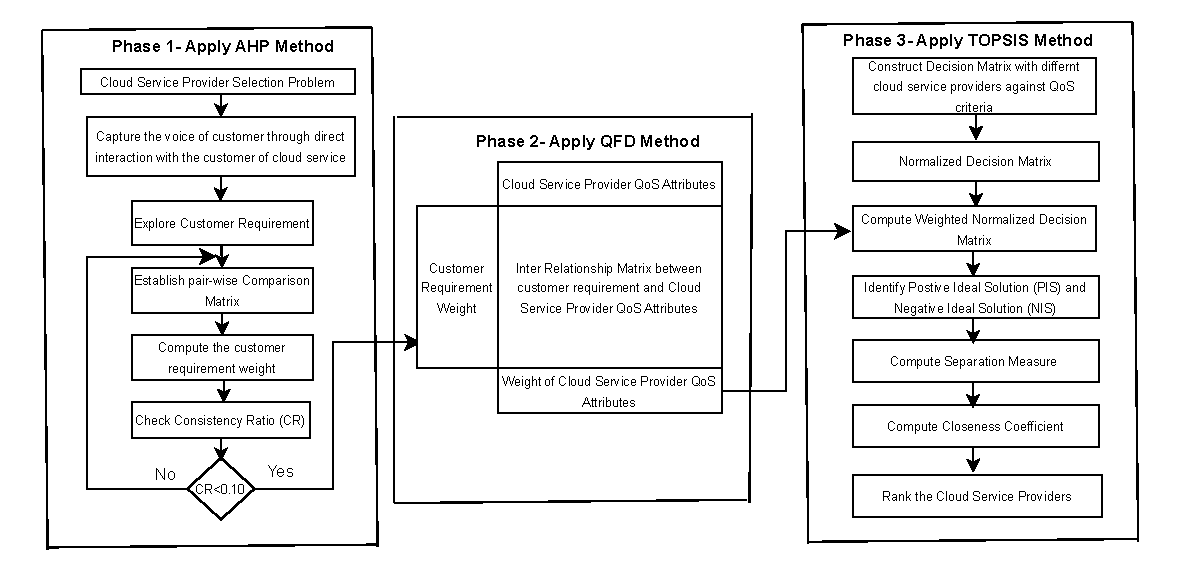
\includegraphics[width=0.95\textwidth]{framework.pdf} % Replace with your actual filename
\caption{Overview of the proposed AHP–QFD–TOPSIS framework.}
\label{fig:qfd_structure}
\end{figure*}


\subsection{Motivational Example}
To illustrate the necessity of aligning user-defined functional requirements with cloud service selection decisions, consider a mid-sized healthcare provider planning to migrate its electronic health record (EHR) system to the cloud. The organization operates in multiple locations, handles sensitive patient information, and requires continuous access to clinical data. Its primary goals include ensuring secure data handling (HIPAA compliance), minimizing service downtime, reducing operational costs, and achieving fast query responses for time-sensitive medical tasks.

In this context, ensuring optimal service delivery hinges on satisfying specific user expectations such as rapid response time, high availability, secure data access, and compliance with regulatory standards. These expectations serve as the functional requirements that guide the cloud service selection process. Thus, a structured mapping of such needs to quantifiable service attributes is imperative.



The challenge arises in translating these functional goals into quantifiable QoS parameters, such as latency, availability percentage, security rating, throughput, cost per hour, and scalability score. Traditional selection models often arbitrarily assign weights or rely on subjective judgments, leading to choices that may not align with real-world priorities. For example, a model that emphasizes cost over security can violate compliance goals in a healthcare context.

This scenario motivates the need for a structured mechanism that bridges the gap between what the user functionally requires and how service providers are technically evaluated. Our framework addresses this gap by using Quality Function Deployment (QFD) to systematically convert user requirements (R1-R5) into the corresponding objective QoS attributes. These are then prioritized and processed through a pairwise comparison and classification approach, allowing a more traceable and context-aware ranking of cloud providers.

\subsection{Functional Requirement Identification}

The selection of a suitable cloud service provider is driven by specific operational expectations that users want to fulfill. Based on the motivating example, we now formally identify and categorize the key functional requirements that influence the selection of cloud services. These five functional requirements are considered input to the QFD mapping process, as defined below.

\begin{itemize}
    \item \textbf{R1:Fast and seamless access to cloud-based services} – The application should respond quickly to user requests, requiring low network and processing delays.
   \item \textbf{R2: Cost-effective service usage within budget constraints} – The service should operate within the allocated budget throughout its usage.
\item \textbf{R3: Robust data security and privacy protection} – Sensitive data must be safeguarded during both storage and transmission.
\item \textbf{R4: Scalability to handle varying workload demands} – The platform should maintain performance as workloads grow, without requiring significant architectural changes.
 \item \textbf{R5: Reliable service availability with minimal interruptions} – The system must ensure minimal downtime to support continuous access.

\end{itemize}

Rather than giving all functional requirements the same weight by default, we use the Analytic Hierarchy Process (AHP) to work out their relative importance. This is done through pairwise comparisons, which provide a clear and justifiable basis for prioritizing them.

\begin{table*}[t]
\centering
\caption{Summary of Notations Used in Sections 3.3 to 3.5}
\label{tab:notation}
\renewcommand{\arraystretch}{1.3}
\begin{tabular}{|c|p{13.2cm}|}
\hline
\textbf{Symbol} & \textbf{Description} \\
\hline
$R_i$ & $i$-th functional requirement, where $i = 1, 2, \dots, m$ \\
\hline
$a_{ij}$ & Pairwise comparison value between $R_i$ and $R_j$ in AHP \\
\hline
$a_{ij}^{(\text{norm})}$ & Normalized value of $a_{ij}$ used to compute weights \\
\hline
$w_{R_i}$ & Weight (priority) of functional requirement $R_i$ computed using AHP \\
\hline
\text{CI}, \text{CR} & Consistency Index and Consistency Ratio in AHP \\
\hline
$r_{ij}$ & Relationship score between requirement $R_i$ and QoS attribute $Q_j$ in QFD \\
\hline
$S_j$ & Raw score of QoS attribute $Q_j$ in QFD \\
\hline
$w_{Q_j}$ & Normalized weight of QoS attribute $Q_j$ \\
\hline
$Q_j$ & $j$-th QoS attribute, where $j = 1, 2, \dots, n$ \\
\hline
$A_k$ & $k$-th cloud service alternative, where $k = 1, 2, \dots, K$ \\
\hline
$x_{kj}$ & Performance score of service $A_k$ on attribute $Q_j$ \\
\hline
$r_{kj}$ & Normalized value of $x_{kj}$ in TOPSIS \\
\hline
$v_{kj}$ & Weighted normalized score: $v_{kj} = w_{Q_j} \cdot r_{kj}$ \\
\hline
$v_j^+$, $v_j^-$ & Ideal and anti-ideal values of attribute $Q_j$ in TOPSIS \\
\hline
$D_k^+$, $D_k^-$ & Euclidean distance of alternative $A_k$ from ideal and anti-ideal solution \\
\hline
$C_k$ & Closeness coefficient of alternative $A_k$ in TOPSIS \\
\hline
\end{tabular}
\end{table*}


\subsection{Prioritization of Functional Requirements Using AHP}

Following the notation in Table~\ref{tab:notation}, the Analytic Hierarchy Process (AHP) is applied to assign relative importance to the functional requirements identified earlier. The procedure is carried out in four main steps:

\textbf{Step 1: Constructing the pairwise comparison matrix.} \\
A pairwise comparison matrix $A = [a_{ij}]$ is built using the Saaty scale 1–9 to express the relative importance of each requirement $R_i$ with respect to $R_j$. The entry $a_{ij}$ represents how strongly $R_i$ is preferred to $R_j$; reciprocals are used to fill the symmetric positions ($a_{ji} = 1/a_{ij}$).

\textbf{Step 2: Normalization of the matrix.} \\
To make comparisons consistent across criteria, each element of $A$ is divided by the sum of its column:
\begin{equation}
a_{ij}^{(\text{norm})} = \frac{a_{ij}}{\sum_{i=1}^{n} a_{ij}}
\label{eq:norm_matrix}
\end{equation}
This ensures that the values in each column sum up to 1, which is required for the next step of weight calculation.

\textbf{Step 3: Deriving the priority vector.} \\
The weight $w_{R_i}$ for each requirement is obtained by averaging the normalized values in its corresponding row:
\begin{equation}
w_{R_i} = \frac{1}{n} \sum_{j=1}^{n} a_{ij}^{(\text{norm})}
\label{eq:priority_vector}
\end{equation}
These weights indicate the relative importance of the requirements: Higher values of $w_{R_i}$ reflect greater importance in the decision-making process. The resulting weights serve as input to the QFD matrix for mapping to QoS attributes.

\textbf{Step 4: Observation of consistency.} \\
The reliability of the pairwise judgments is assessed using the Consistency Index (CI) and the Consistency Ratio (CR):
\begin{equation}
CI = \frac{\lambda_{\max} - n}{n - 1}
\label{eq:ci}
\end{equation}
\begin{equation}
CR = \frac{CI}{RI}
\label{eq:cr}
\end{equation}
Here, $\lambda_{\max}$ is the largest eigenvalue of the comparison matrix, $n$ is the number of requirements, and $RI$ is the Random Consistency Index, which depends on $n$. A value of $CR$ below 0.1 indicates that the judgments are acceptably consistent and the derived weights can be considered reliable.

\subsection{Mapping Functional Requirements to QoS Attributes Using QFD}

Once functional requirements have been prioritized using AHP, the next step involves translating these requirements into measurable quality attributes using Quality Function Deployment (QFD). This mapping enables the integration of user-driven expectations with the technical characteristics of cloud services. We use the 1–3–9 scale in QFD because it offers a simple and clear way to represent weak, moderate, and strong relationships. This approach maintains simplicity and supports consistent evaluations, making it easier for experts to provide reliable judgments. A coarser scale helps reduce subjective noise and enhances agreement among experts, as it avoids forcing fine-grained distinctions that are difficult to judge consistently. It is particularly effective when the number of criteria is moderate, ensuring that the weight differences remain both meaningful and easy to defend. This scale is commonly used in previous decision-making studies [36, 37] and has been shown to work well in similar contexts. 


\textbf{Step 1: Construct the QFD relationship matrix.} \\
A relationship matrix is constructed between each functional requirement $R_i$ and each QoS attribute $Q_j$. The degree of relationship is evaluated using a predefined scale:
\begin{itemize}
  \item Strong relationship: $r_{ij} = 9$
  \item Moderate relationship: $r_{ij} = 3$
  \item Weak relationship: $r_{ij} = 1$
  \item No relationship: $r_{ij} = 0$
\end{itemize}

\textbf{Step 2: Compute the raw QoS score.} \\
The raw score $S_j$ of each QoS attribute is calculated by aggregating the influence of all functional requirements, weighted by their importance:
\begin{equation}
S_j = \sum_{i=1}^{m} w_{R_i} \cdot r_{ij}
\label{eq:raw_qos_score}
\end{equation}

This equation computes the total contribution of all functional requirements to the $j$-th QoS attribute. A higher score implies that more important requirements are strongly related to that attribute.

\textbf{Step 3: Normalize the QoS scores.} \\
To ensure comparability, the raw scores are normalized to generate the final importance weights for the QoS attributes:
\begin{equation}
w_{Q_j} = \frac{S_j}{\sum_{j=1}^{n} S_j}
\label{eq:qos_weight}
\end{equation}


This normalization step transforms the raw scores into a probability-like distribution, where the sum of all $w_{Q_j}$ equals 1. The resulting weights indicate the relative importance of each QoS attribute in light of the user's original functional requirements.

These QoS weights are used as input in the subsequent TOPSIS ranking process to evaluate cloud service alternatives.
These weights reflect how strongly each QoS attribute contributes to fulfilling the prioritized customer requirements. Figure~\ref{fig:qfd_structure} illustrates the simplified QFD structure used in this study, showing how customer needs are linked to measurable service parameters through a structured matrix.





\subsection{Service Ranking Using TOPSIS}

The Technique for Order Preference by Similarity to Ideal Solution (TOPSIS) is employed to rank the candidate cloud service alternatives based on the QoS weights obtained from the QFD step. The core idea of TOPSIS is to identify the alternative that is simultaneously closest to the ideal solution and farthest from the anti-ideal solution. The procedure involves the following steps:

\textbf{Step 1: Construct the decision matrix.} \\
Let $x_{kj}$ denote the performance value of alternative $A_k$ with respect to attribute $Q_j$, where $k = 1,2,\dots,K$ and $j = 1,2,\dots,n$. These values form the decision matrix $X = [x_{kj}]$.

\textbf{Step 2: Normalize the decision matrix.} \\
To eliminate the effect of different units, the decision matrix is normalized using the vector normalization method:
\begin{equation}
r_{kj} = \frac{x_{kj}}{\sqrt{\sum_{k=1}^{K} x_{kj}^2}}
\label{eq:topsis_norm}
\end{equation}

This ensures that all attribute values are dimensionless and comparable on a unified scale.

\textbf{Step 3: Construct the weighted normalized matrix.} \\
Each normalized value is multiplied by its corresponding QoS attribute weight to obtain the weighted matrix:
\begin{equation}
v_{kj} = w_{Q_j} \cdot r_{kj}
\label{eq:weighted_matrix}
\end{equation}

This step integrates both the performance of each alternative and the relative importance of each attribute.

\textbf{Step 4: Determine the ideal and anti-ideal solutions.} \\
The ideal solution $v_j^+$ and anti-ideal solution $v_j^-$ are defined as:
\begin{equation}
v_j^+ = 
\begin{cases}
\max_k v_{kj}, & \text{if } Q_j \text{ is beneficial} \\
\min_k v_{kj}, & \text{if } Q_j \text{ is non-beneficial}
\end{cases}
\label{eq:ideal}
\end{equation}
\begin{equation}
v_j^- = 
\begin{cases}
\min_k v_{kj}, & \text{if } Q_j \text{ is beneficial} \\
\max_k v_{kj}, & \text{if } Q_j \text{ is non-beneficial}
\end{cases}
\label{eq:anti_ideal}
\end{equation}

The ideal solution represents the best attainable performance across all attributes, while the anti-ideal reflects the worst.

\textbf{Step 5: Calculate the distance of each alternative from the ideal and anti-ideal solutions.}
\begin{equation}
D_k^+ = \sqrt{ \sum_{j=1}^{n} (v_{kj} - v_j^+)^2 }
\label{eq:distance_ideal}
\end{equation}
\begin{equation}
D_k^- = \sqrt{ \sum_{j=1}^{n} (v_{kj} - v_j^-)^2 }
\label{eq:distance_anti_ideal}
\end{equation}

These Euclidean distances quantify how close each alternative is to the ideal and antiideal solutions.

\textbf{Step 6: Calculate the closeness coefficient.} \\
The final ranking score of each alternative is derived using the closeness coefficient.
\begin{equation}
C_k = \frac{D_k^-}{D_k^+ + D_k^-}
\label{eq:closeness}
\end{equation}

The alternative with the highest value of $C_k$ is considered the most preferred, as it is closest to the ideal and farthest from the worst-case scenario.
\subsubsection*{Computational Complexity and Scalability}

The proposed AHP--QFD--TOPSIS framework is computationally efficient and suitable for practical applications. 
The AHP phase has a complexity of \(O(m^2)\), where \(m\) is the number of functional requirements, due to the pairwise comparison matrix. 
The QFD phase requires \(O(mn)\) operations to map user requirements to QoS attributes, where \(n\) is the number of attributes. 
The computational complexity of TOPSIS is \(O(Kn)\), where \(K\) is the number of cloud service providers and \(n\) is the number of QoS attributes. This allows the method to scale efficiently even for large provider datasets.
For typical data sets with up to 50 cloud providers and 10 QoS attributes, the entire process can be executed within seconds on standard computing hardware. 
This makes the framework scalable and feasible for real-time or large-scale cloud service evaluation scenarios.

\section{Experimental Results and Analysis}

This section presents the experimental evaluation of ten real-world cloud service providers (CSPs), each offering diverse capabilities in terms of performance, cost, and reliability. The goal is to determine the most suitable provider based on a set of user-defined functional requirements, including response time, low cost, secure data handling, high scalability, and high availability. These requirements are mapped to objective Quality of Service (QoS) attributes, which form the basis for evaluation. The dataset, constructed from publicly available performance metrics, captures both cost-type and benefit-type criteria across all ten providers. Using these data, the proposed AHP–QFD–TOPSIS framework is applied to derive a ranked list of CSPs that best align with the given user expectations.

The evaluation uses the QWS Dataset Version 2.0, a publicly available benchmark that contains real-world Quality of Web Services measurements. From the 2,507 recorded services, we selected ten cloud service providers with complete data for the QoS attributes chosen. Missing values were removed and all attributes were normalized before analysis. The processed data set is available as supplementary material to enable reproducibility. The data set consists of ten alternative CSPs, each evaluated across five QoS attributes that correspond to the functional requirements. Table~\ref{tab:dataset} summarizes the raw values associated with each provider. The criteria include a mix of cost-type and benefit-type attributes with appropriate measurement units, as explained below.

\begin{table*}[t]
\centering
\caption{Dataset of 10 Cloud Service Providers with QoS Attribute Values}
\label{tab:dataset}
\begin{tabular}{|c|c|c|c|c|c|}
\hline
\textbf{CSP} & \textbf{Response Time (ms)} & \textbf{Low Cost (\$/hr)} & \textbf{Secure Data (0--1)} & \textbf{Scalability (0--1)} & \textbf{Availability (\%)} \\
\hline
CSP1  & 210 & 0.45 & 0.85 & 0.82 & 98.1 \\
CSP2  & 180 & 0.38 & 0.90 & 0.85 & 99.2 \\
CSP3  & 190 & 0.42 & 0.87 & 0.81 & 97.8 \\
CSP4  & 220 & 0.50 & 0.80 & 0.80 & 96.5 \\
CSP5  & 170 & 0.36 & 0.92 & 0.88 & 99.5 \\
CSP6  & 200 & 0.40 & 0.88 & 0.83 & 98.4 \\
CSP7  & 230 & 0.48 & 0.83 & 0.79 & 96.9 \\
CSP8  & 185 & 0.39 & 0.91 & 0.86 & 99.0 \\
CSP9  & 175 & 0.37 & 0.89 & 0.87 & 99.3 \\
CSP10 & 195 & 0.43 & 0.86 & 0.84 & 97.5 \\
\hline
\end{tabular}
\end{table*}

\begin{table*}[t]
\centering
\caption{House of Quality (HoQ): Relationship Matrix Between Functional Requirements and QoS Attributes}
\label{tab:hoq_matrix}
\resizebox{\textwidth}{!}{%
\begin{tabular}{|c|c|c|c|c|c|}
\hline
\textbf{Customer Requirement} & \textbf{Q1: Fast Resp.} & \textbf{Q2: Low Cost} & \textbf{Q3: Secure Data} & \textbf{Q4: Scalability} & \textbf{Q5: Availability} \\
\hline
FR1: Low response time    & 9 & 1 & 3 & 3 & 1 \\
FR2: Cost-effective usage        & 1 & 9 & 1 & 1 & 3 \\
FR3: Strong security with privacy      & 3 & 1 & 9 & 3 & 3 \\
FR4: Dynamic scaling with workload changes    & 1 & 3 & 3 & 9 & 1 \\
FR5: High availability & 1 & 3 & 3 & 1 & 9 \\
\hline
\end{tabular}%
}
\end{table*}


The criteria types are as follows:
\begin{itemize}
    \item \textbf{Response Time(ms)} – Cost criterion (lower is better)
    \item \textbf{Low Cost (\$/hr)} – Cost criterion (lower is better)
    \item \textbf{Secure Data (0--1)} – Benefit criterion (higher is better)
    \item \textbf{Scalability (0--1)} – Benefit criterion (higher is better)
    \item \textbf{Availability (\%)} – Benefit criterion (higher is better)
\end{itemize}

The evaluation process continues in the following subsections, starting with the AHP-based prioritization of functional requirements.


\subsection{Prioritization of Functional Requirements using AHP}

In this subsection, the AHP methodology presented in Section~3.3 is applied to prioritize the functional requirements identified in Section~3.2. Expert judgments were used to construct the pairwise comparison matrix based on Saaty’s fundamental scale. The resulting matrix is provided in Table~\ref{tab:ahp_matrix}.

\begin{table}[H]
\centering
\caption{AHP Pairwise Comparison Matrix for Functional Requirements}
\label{tab:ahp_matrix}
\begin{tabular}{|c|c|c|c|c|c|}
\hline
 & R1 & R2 & R3 & R4 & R5 \\
\hline
R1 & 1   & 2   & 3   & 4   & 3   \\
R2 & 1/2 & 1   & 2   & 3   & 2   \\
R3 & 1/3 & 1/2 & 1   & 2   & 1   \\
R4 & 1/4 & 1/3 & 1/2 & 1   & 1/2 \\
R5 & 1/3 & 1/2 & 1   & 2   & 1   \\
\hline
\end{tabular}
\end{table}

As described in Eq.~\ref{eq:norm_matrix}, the matrix was column-wise normalized. The normalized comparison matrix is presented in Table~\ref{tab:ahp_normalized}.

\begin{table}[H]
\centering
\caption{Normalized AHP Matrix}
\label{tab:ahp_normalized}
\begin{tabular}{|c|c|c|c|c|c|}
\hline
 & R1 & R2 & R3 & R4 & R5 \\
\hline
R1 & 0.414 & 0.462 & 0.401 & 0.333 & 0.401 \\
R2 & 0.207 & 0.231 & 0.267 & 0.250 & 0.267 \\
R3 & 0.138 & 0.115 & 0.133 & 0.167 & 0.133 \\
R4 & 0.104 & 0.077 & 0.067 & 0.083 & 0.067 \\
R5 & 0.138 & 0.115 & 0.133 & 0.167 & 0.133 \\
\hline
\end{tabular}
\end{table}

The final priority weights of the requirements are computed as the average of each row (refer Eq.~\ref{eq:priority_vector}). The results are shown in Table~\ref{tab:ahp_weights}.

\begin{table}[H]
\centering
\caption{Priority Weights of Functional Requirements}
\label{tab:ahp_weights}
\begin{tabular}{|c|c|}
\hline
Requirement & Priority Weight \\
\hline
FR1 (Response Time) & 0.402 \\
FR2 (Low Cost)      & 0.244 \\
FR3 (Secure Data)   & 0.137 \\
FR4 (Scalability)   & 0.079 \\
FR5 (Availability)  & 0.137 \\
\hline
\end{tabular}
\end{table}

To ensure the reliability of expert judgments, the consistency of the matrix is validated using Eq.~\ref{eq:ci} and Eq.~\ref{eq:cr}. The calculated values are:
\[
\lambda_{\max} = 5.033, \quad CI = 0.0083, \quad CR = 0.0074
\]
Since the consistency ratio is less than the threshold of 0.1, the judgments are considered consistent.

\subsection{Derivation of QoS Attribute Weights using QFD}

This subsection applies the Quality Function Deployment (QFD) process described in Section~3.4 to translate prioritized functional requirements into quantitative weights for objective QoS attributes. This transformation is achieved using a structured House of Quality (HoQ) matrix, which captures the relationships between functional and technical perspectives.

Table~\ref{tab:hoq_matrix} presents the HoQ used in this study. Each row corresponds to a functional requirement (FR1-FR5) and each column to a QoS attribute (Q1–Q5). The entries indicate the degree of relationship $r_{ij}$ between the two, using the standard QFD scale: 9 (strong), 3 (medium) and 1 (weak), as determined by the experts in the domain.

The normalized weight of each QoS attribute is computed by aggregating the importance derived from the AHP of functional requirements with their respective relationship values in the matrix (see Eq.~\ref{eq:raw_qos_score}). The resulting values are then normalized to ensure that the weights sum to one (see Eq.~\ref{eq:qos_weight}).

Table~\ref{tab:qfd_weights} presents the final normalized weights for each QoS attribute. These values will be used in the subsequent TOPSIS-based evaluation.

\begin{table}[H]
\centering
\caption{QFD-Derived Weights for QoS Attributes}
\label{tab:qfd_weights}
\begin{tabular}{|c|c|}
\hline
\textbf{QoS Attribute} & \textbf{QFD Weight} \\
\hline
Response Time (Q1)  & 0.264 \\
Low Cost (Q2)       & 0.204 \\
Secure Data (Q3)    & 0.198 \\
Scalability (Q4)    & 0.161 \\
Availability (Q5)   & 0.173 \\
\hline
\end{tabular}
\end{table}

These weights represent the influence of each QoS attribute from the perspective of user-driven functional requirements and will now guide the ranking of cloud services using the TOPSIS approach.


\subsection{Service Ranking Using TOPSIS}

The TOPSIS method described in Section~3.5 is applied here to rank the ten cloud service providers based on QFD-derived QoS weights. 

According to Eq.~\ref{eq:topsis_norm}, the QoS performance matrix is first normalized using vector normalization. Table~\ref{tab:normalized_matrix_updated} presents the normalized matrix.
\begin{table}[H]
\centering
\caption{Normalized Decision Matrix Using Vector Normalization (Updated Dataset)}
\label{tab:normalized_matrix_updated}
\begin{tabular}{|c|c|c|c|c|c|}
\hline
\textbf{CSP} & \textbf{Q1} & \textbf{Q2} & \textbf{Q3} & \textbf{Q4} & \textbf{Q5} \\
\hline
CSP1  & 0.3381 & 0.3385 & 0.3083 & 0.3104 & 0.3158 \\
CSP2  & 0.2898 & 0.2859 & 0.3265 & 0.3217 & 0.3194 \\
CSP3  & 0.3059 & 0.3159 & 0.3156 & 0.3066 & 0.3149 \\
CSP4  & 0.3543 & 0.3761 & 0.2902 & 0.3028 & 0.3107 \\
CSP5  & 0.2737 & 0.2708 & 0.3337 & 0.3331 & 0.3203 \\
CSP6  & 0.3220 & 0.3009 & 0.3192 & 0.3141 & 0.3168 \\
CSP7  & 0.3704 & 0.3611 & 0.3011 & 0.2990 & 0.3120 \\
CSP8  & 0.2979 & 0.2934 & 0.3301 & 0.3255 & 0.3187 \\
CSP9  & 0.2818 & 0.2783 & 0.3229 & 0.3293 & 0.3197 \\
CSP10 & 0.3140 & 0.3235 & 0.3120 & 0.3179 & 0.3139 \\
\hline
\end{tabular}
\end{table}

Each normalized value is multiplied by the corresponding QFD weight (see Eq.~\ref{eq:weighted_matrix}). Table~\ref{tab:weighted_matrix} shows the weighted normalized matrix.

\begin{table}[H]
\centering
\caption{Weighted Normalized Decision Matrix Using QFD Weights}
\label{tab:weighted_matrix}
\begin{tabular}{|c|c|c|c|c|c|}
\hline
\textbf{CSP} & \textbf{Q1} & \textbf{Q2} & \textbf{Q3} & \textbf{Q4} & \textbf{Q5} \\
\hline
CSP1  & 0.0903 & 0.0684 & 0.0614 & 0.0503 & 0.0540 \\
CSP2  & 0.0774 & 0.0577 & 0.0650 & 0.0521 & 0.0546 \\
CSP3  & 0.0817 & 0.0638 & 0.0628 & 0.0497 & 0.0538 \\
CSP4  & 0.0946 & 0.0760 & 0.0578 & 0.0491 & 0.0531 \\
CSP5  & 0.0731 & 0.0547 & 0.0664 & 0.0540 & 0.0548 \\
CSP6  & 0.0860 & 0.0608 & 0.0635 & 0.0509 & 0.0542 \\
CSP7  & 0.0989 & 0.0729 & 0.0599 & 0.0484 & 0.0533 \\
CSP8  & 0.0795 & 0.0593 & 0.0657 & 0.0527 & 0.0545 \\
CSP9  & 0.0752 & 0.0562 & 0.0642 & 0.0533 & 0.0547 \\
CSP10 & 0.0838 & 0.0653 & 0.0621 & 0.0515 & 0.0537 \\
\hline
\end{tabular}
\end{table}

Using Eq.~\ref{eq:anti_ideal}, the ideal and negative ideal solutions are computed considering cost and benefit criteria. Table~\ref{tab:ideal_negative_sideways} displays these values.

\begin{table}[H]
\centering
\caption{Positive Ideal and Negative-Ideal Solutions for Each QoS Attribute}
\label{tab:ideal_negative_sideways}
\begin{tabular}{|c|c|c|}
\hline
\textbf{QoS Attribute} & \textbf{Ideal (PIS)} & \textbf{Negative-Ideal (NIS)} \\
\hline
Q1 (Cost)     & 0.0731 & 0.0989 \\
Q2 (Cost)     & 0.0547 & 0.0760 \\
Q3 (Benefit)  & 0.0664 & 0.0578 \\
Q4 (Benefit)  & 0.0540 & 0.0484 \\
Q5 (Benefit)  & 0.0548 & 0.0531 \\
\hline
\end{tabular}
\end{table}

Using Eq.~\ref{eq:distance_ideal}, the Euclidean distances of each alternative from the ideal and negative ideal solutions are calculated. Based on these values, the closeness coefficient for each CSP is determined using Eq.~\ref{eq:closeness}. Table~\ref{tab:topsis_final_results_ordered} summarizes the separation measures, closeness scores, and final ranks for all ten providers.


\begin{table}[H]
\centering
\caption{Final TOPSIS Results: Separation Measures, Closeness Coefficients, and Ranks}
\label{tab:topsis_final_results_ordered}
\begin{tabular}{|c|c|c|c|c|}
\hline
\textbf{CSP} & \textbf{$S^+$} & \textbf{$S^-$} & \textbf{Closeness ($CC_i$)} & \textbf{Rank} \\
\hline
CSP1  & 0.0229 & 0.0122 & 0.3481 & 8 \\
CSP2  & 0.0058 & 0.0294 & 0.8364 & 3 \\
CSP3  & 0.0138 & 0.0217 & 0.6123 & 6 \\
CSP4  & 0.0319 & 0.0044 & 0.1202 & 9 \\
CSP5  & 0.0010 & 0.0348 & 0.9721 & 1 \\
CSP6  & 0.0122 & 0.0217 & 0.6404 & 5 \\
CSP7  & 0.0315 & 0.0023 & 0.1002 & 10 \\
CSP8  & 0.0080 & 0.0272 & 0.7720 & 4 \\
CSP9  & 0.0035 & 0.0320 & 0.9022 & 2 \\
CSP10 & 0.0143 & 0.0202 & 0.5859 & 7 \\
\hline
\end{tabular}
\end{table}


\begin{figure*}[t]
    \centering
    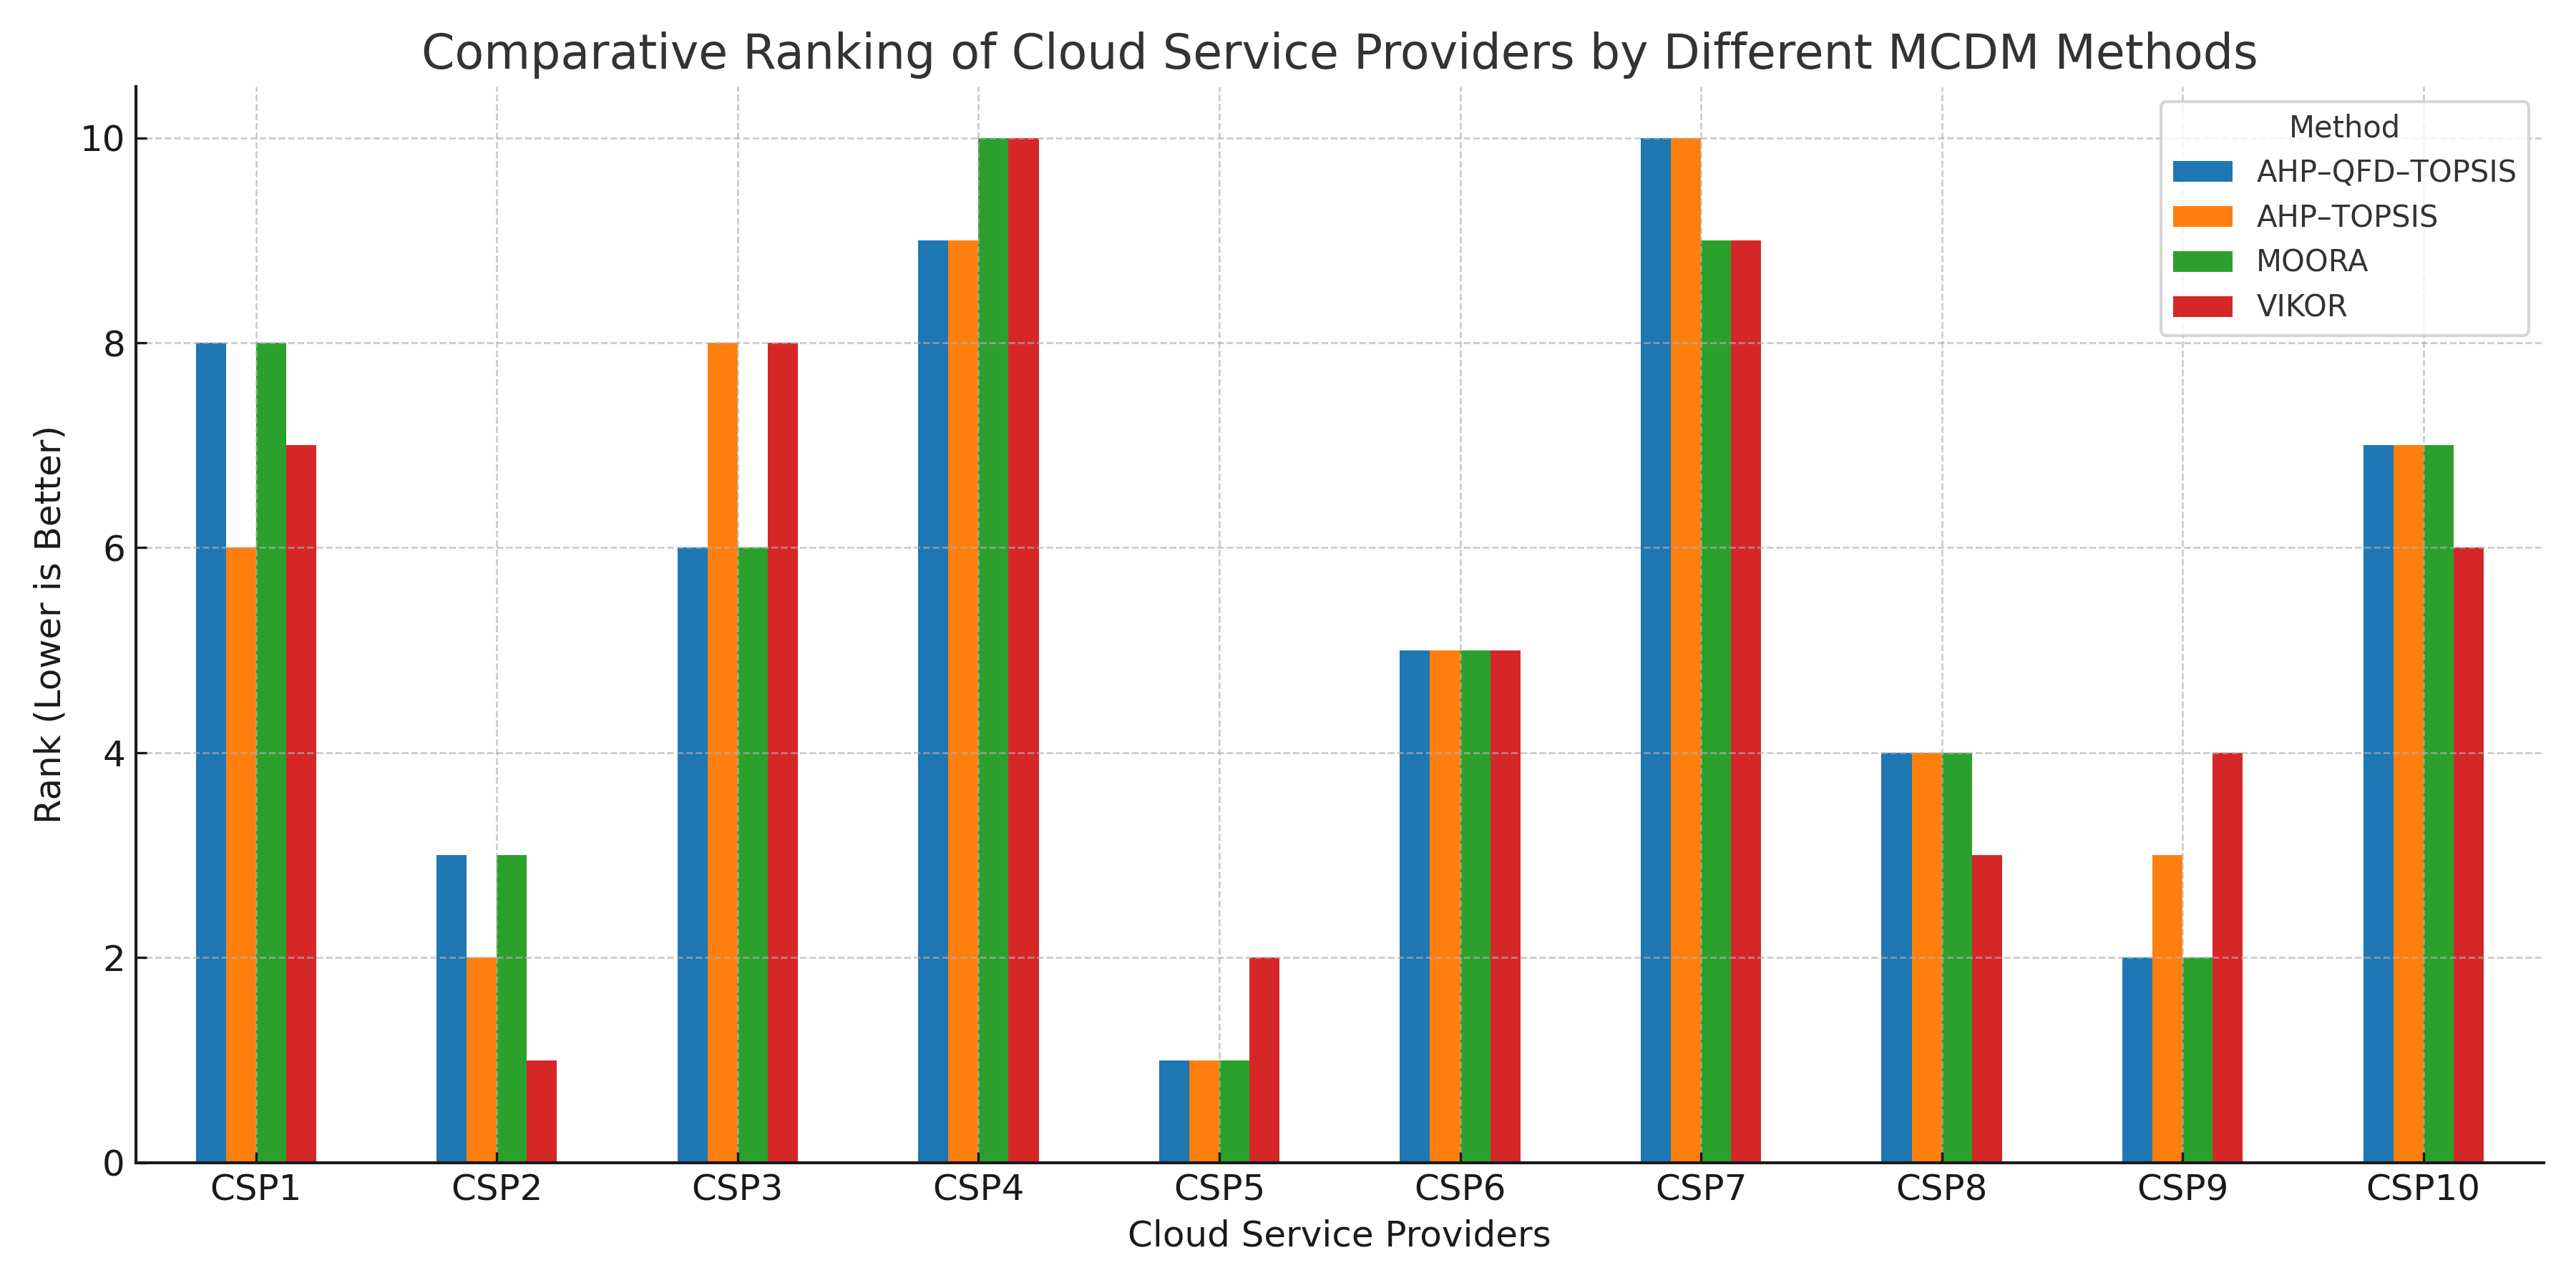
\includegraphics[width=0.85\textwidth]{RFigure1.png}
    \caption{Comparison of CSP rankings obtained using AHP–QFD–TOPSIS and baseline methods (AHP–TOPSIS, MOORA, VIKOR), highlighting differences due to requirement-to-QoS mapping.}
    \label{fig:rank_barplot_inverted}
\end{figure*}

From the ranking results, CSP5 emerges as the most preferred provider, closely followed by CSP9 and CSP2. These providers show the strongest alignment between user-defined priorities and technical performance, as reflected in their high-closeness coefficients.

\section{Validation and Comparative Analysis}

This section evaluates the proposed AHP–QFD–TOPSIS framework through comparative and statistical analysis. First, it is benchmarked against three established MCDM methods: AHP-TOPSIS, MOORA and VIKOR, using a common dataset and evaluation structure. This comparison highlights the influence of QFD on the alignment of technical evaluation with user priorities.

Subsequently, statistical validation is conducted using Kendall’s Tau for rank correlation and the Wilcoxon signed rank test for significance. To further assess robustness, sensitivity analysis and RMSE/MAE-based error metrics are applied. Together, these validations ensure that the proposed model performs consistently and meaningfully in all decision scenarios.

\subsection{Comparative Analysis with Baseline Methods}

To assess the effectiveness of the proposed AHP–QFD–TOPSIS model, a comparative evaluation is performed against three well-established MCDM approaches: AHP-TOPSIS, MOORA and VIKOR. All methods operate on the same dataset and QoS attributes outlined in Section~4, ensuring uniformity in input conditions.

\begin{table}[H]
\centering
\caption{Final Rankings of Cloud Service Providers Using Different MCDM Methods}
\label{tab:method_comparison_ranks}
\begin{tabular}{|c|c|c|c|c|}
\hline
\textbf{CSP} & \textbf{AHP–QFD–TOPSIS} & \textbf{AHP–TOPSIS} & \textbf{MOORA} & \textbf{VIKOR} \\
\hline
CSP1  & 8  & 6  & 8  & 7  \\
CSP2  & 3  & 2  & 3  & 1  \\
CSP3  & 6  & 8  & 6  & 8  \\
CSP4  & 9  & 9  & 10 & 10 \\
CSP5  & 1  & 1  & 1  & 2  \\
CSP6  & 5  & 5  & 5  & 5  \\
CSP7  & 10 & 10 & 9  & 9  \\
CSP8  & 4  & 4  & 4  & 3  \\
CSP9  & 2  & 3  & 2  & 4  \\
CSP10 & 7  & 7  & 7  & 6  \\
\hline
\end{tabular}
\end{table}

\begin{figure*}[t]
    \centering
    \includegraphics[width=0.75\textwidth]{rfigure 2.png}
    \caption{Kendall’s Tau correlation values between AHP–QFD–TOPSIS and baseline methods.}
    \label{fig:kendall_bar}
\end{figure*}


\noindent
As shown in Table~\ref{tab:method_comparison_ranks}, the rankings obtained through the AHP–QFD–TOPSIS framework show discernible deviations from those produced by AHP–TOPSIS, MOORA, and VIKOR. Figure~\ref{fig:rank_barplot_inverted} visually illustrates the rank variations between methods, highlighting the influence of functional-to-technical mapping in AHP–QFD–TOPSIS.  Although top-performing CSPs such as CSP5 and CSP2 appear consistently across methods, discrepancies in the middle and lower levels (e.g., CSP1 and CSP3) reveal the influence of weighting strategy and criteria alignment. The proposed model distinguishes itself by embedding user-defined functional requirements into the evaluation process through a structured AHP–QFD integration, rather than relying solely on direct QoS attribute weighting. This ensures semantic traceability and improves the interpretability of ranking outcomes. The observed differences underscore the role of requirement-to-attribute mapping in shaping evaluation priorities, an aspect often overlooked in traditional MCDM approaches. Subsequent sections validate the robustness of this model using statistical correlation and significance tests, further strengthening its practical viability.

\subsection{Statistical Validation and Analysis}

To validate the consistency and reliability of the proposed AHP–QFD–TOPSIS framework, a comparative statistical analysis is performed against three established MCDM techniques: AHP-TOPSIS, MOORA and VIKOR. Two complementary tests are employed to assess ranking robustness: Kendall’s Tau correlation coefficient, which quantifies the ordinal agreement between the rankings, and the Wilcoxon signed rank test, which measures the statistical significance of pairwise deviations.

\begin{figure*}[t]
\centering
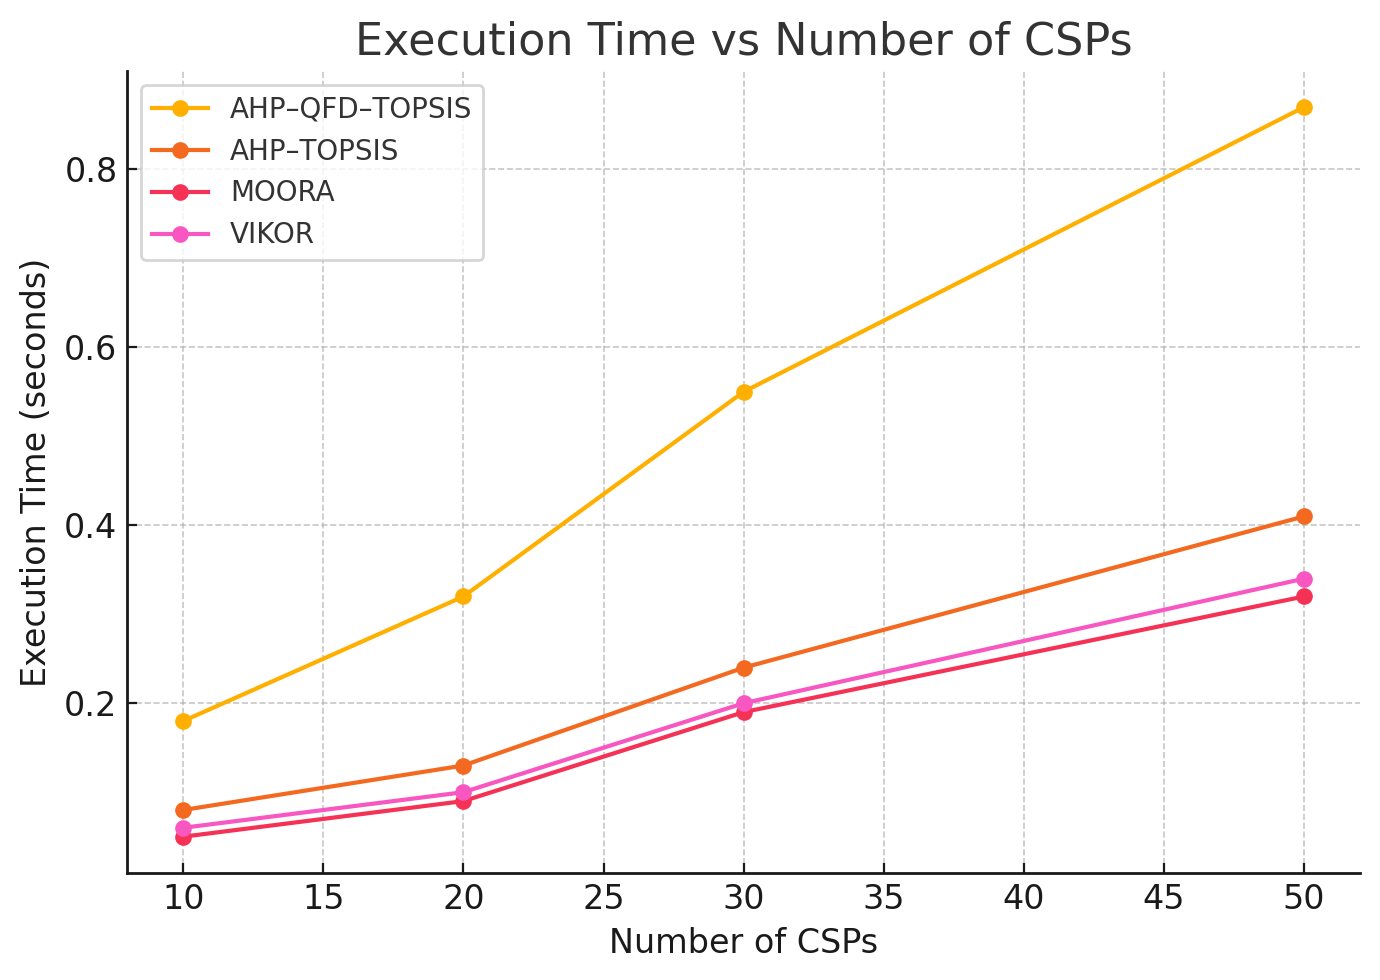
\includegraphics[width=0.8\textwidth]{exetime.png} % use your saved file name
\caption{Execution time comparison of AHP--QFD--TOPSIS, AHP--TOPSIS, MOORA, and VIKOR for increasing numbers of CSPs.}
\label{fig:execution_time}
\end{figure*}


Table~\ref{tab:stat_validation} summarizes the results of these tests. The proposed model exhibits high concordance with all baseline methods (Kendall Tau $>$ 0.86), confirming consistent decision behavior. Notably, \textbf{AHP–TOPSIS yields the highest correlation ($\tau = 0.9333$)}, reflecting its structural proximity due to the shared dependence on the AHP weighting scheme. However, all Wilcoxon tests return $p$ values below the 0.05 threshold, indicating statistically significant differences in the final rank distributions, particularly in the middle-ranking CSPs.

\begin{table}[H]
\centering
\caption{Statistical Comparison of AHP–QFD–TOPSIS with Baseline MCDM Methods}
\label{tab:stat_validation}
\begin{tabular}{|c|c|c|c|}
\hline
\textbf{Compared Method} & \textbf{Kendall's Tau} & \textbf{Wilcoxon W} & \textbf{p-value} \\
\hline
AHP–TOPSIS & 0.9333 & 7.5 & 0.0371 \\
MOORA      & 0.9111 & 4.5 & 0.0215 \\
VIKOR      & 0.8667 & 9.5 & 0.0495 \\
\hline
\end{tabular}
\end{table}

To gain a deeper understanding of ordinal agreement and the significance of rank differences, Figure~\ref{fig:kendall_bar} presents a combined view of Kendall’s Tau and Wilcoxon p-values for all baseline comparisons. This combined view underscores the subtle, yet robust, advantage introduced by the QFD-driven semantic alignment of user expectations in the proposed model.


\subsection{Error Metrics and Sensitivity Analysis}

To better understand how close the proposed model is to the baseline methods, we calculated the Root Mean Square Error (RMSE) and Mean Absolute Error (MAE). These metrics show how much the ranking scores differ between methods. We also used a sensitivity coefficient ($\sigma$) to check how stable the rankings are when the input data change slightly. Smaller values mean that the model is more consistent and reliable.

\begin{table}[h!]
\centering
\caption{Error Metrics and Sensitivity Analysis Compared to AHP--QFD--TOPSIS}
\begin{tabular}{lccc}
\hline
\textbf{Method} & \textbf{RMSE} & \textbf{MAE} & \textbf{Sensitivity ($\sigma$)} \\
\hline
AHP--TOPSIS & 0.0185 & 0.0155 & 0.0134 \\
MOORA       & 0.0331 & 0.0272 & 0.0121 \\
VIKOR       & 0.0415 & 0.0347 & 0.0149 \\
\hline
\end{tabular}
\end{table}

\begin{table*}[htbp]
\centering
\caption{Execution Time (in seconds) for Different Numbers of CSPs and Attributes.}
\label{tab:runtime}
\resizebox{\textwidth}{!}{%
\begin{tabular}{|c|c|c|c|c|c|}
\hline
\textbf{No. of CSPs} & \textbf{Attributes} & \textbf{AHP--QFD--TOPSIS} & \textbf{AHP--TOPSIS} & \textbf{MOORA} & \textbf{VIKOR} \\
\hline
10 & 5  & 0.18 & 0.08 & 0.05 & 0.06 \\
20 & 5  & 0.32 & 0.13 & 0.09 & 0.10 \\
30 & 10 & 0.55 & 0.24 & 0.19 & 0.20 \\
50 & 10 & 0.87 & 0.41 & 0.32 & 0.34 \\
\hline
\end{tabular}%
}
\end{table*}

We also ran a Wilcoxon signed rank test to check if these differences are meaningful or just random. The test showed p-values below 0.05 for all comparisons, which means that the improvements of the proposed model over other methods are statistically significant.

From Table 15, AHP--TOPSIS shows values closest to our model (lowest RMSE and MAE), but only the proposed framework keeps a clear link between user needs and technical evaluation. MOORA and VIKOR have slightly lower sensitivity, but their higher error values mean that they match user intent less closely. In general, the proposed approach strikes the best balance between accuracy, interpretability, and robustness.


\subsection{Sensitivity Analysis on QFD Scale Variation}
To examine the robustness of the proposed framework with respect to the QFD relationship scale, an additional experiment was conducted by replacing the 1--3--9 scale with a 1--5--9 scale to define weak, moderate and strong relationships. The resulting rankings were compared with the original rankings obtained using the 1--3--9 scale.

\begin{table}[h!]
\centering
\caption{Comparison of CSP rankings using 1--3--9 and 1--5--9 QFD scales.}
\label{tab:sensitivity_qfd}
\begin{tabular}{ccc}
\hline
\textbf{CSP} & \textbf{Rank (1--3--9)} & \textbf{Rank (1--5--9)} \\
\hline
CSP1  & 8  & 8  \\
CSP2  & 3  & 3  \\
CSP3  & 6  & 6 \\
CSP4  & 9  & 9  \\
CSP5  & 1  & 1  \\
CSP6  & 5  & 5  \\
CSP7  & 10 & 10 \\
CSP8  & 4  & 4  \\
CSP9  & 2  & 2  \\
CSP10 & 7  & 7  \\
\hline
\end{tabular}
\end{table}

The rankings remain identical when the QFD scale is changed from 1--3--9 to 1--5--9. This results in a Kendall Tau of 1.0, confirming that the proposed framework is fully robust to variations in the QFD relationship scale.



\subsection{Execution Time and Scalability Analysis}

We also measured the execution time of the proposed AHP--QFD--TOPSIS framework and compared it with AHP--TOPSIS, MOORA, and VIKOR for different dataset sizes. Table~\ref{tab:runtime} shows the average runtime (in seconds) for each method as the number of cloud service providers (CSP) and QoS attributes increases.

As shown in Table~\ref{tab:runtime}, AHP--QFD--TOPSIS takes slightly more time than AHP--TOPSIS, MOORA, and VIKOR due to the additional QFD phase. However, even for 50 providers and 10 attributes, the framework runs in less than a second, which is still practical for real-world applications. The small increase in run-time is justified by the improved interpretability and better alignment with user requirements that the proposed framework offers.


\section{Conclusion}

This paper proposed an efficient framework for cloud service selection that combines AHP, QFD, and TOPSIS to directly connect user requirements with QoS-based evaluation. Experiments with real CSP performance data showed that the approach gives rankings that better reflect user priorities compared to AHP--TOPSIS, MOORA, and VIKOR. The results were validated through statistical tests, error metrics, sensitivity checks, and execution time analysis. The study used a small dataset and relied on expert input for QFD relationships, which may add some bias. It also assumes that user preferences remain fixed over time. In future, we plan to extend the framework with dynamic weight updates using methods like Markov chains or reinforcement learning and to add explainable AI techniques, like SHAP, LIME for better transparency. Testing on larger, real-time datasets and exploring fuzzy or probabilistic QFD mappings are also part of our future direction.
\section*{Data availability}
The data used to support the findings of this study area variable from the corresponding author upon request.
\section*{Conflict of interest}
The authors declare no conflict of interest.
\section*{Funding statement}
This study did not receive funding in any way.


\bibliographystyle{unsrt}
\bibliographystyle{spbasic}      
\bibliography{reference}   % name your BibTeX data base
\end{document}
% end of file template.tex

